\section{Überblick über Open Innovation}\label{sec:grundlagen-open}

Das Modell der \textit{Open Innovation} ist der Gegensatz der \textit{Closed Innovation}.
Da der Fokus dieser Arbeit auf letzterem liegt,
wird im Folgenden der offene Ansatz lediglich oberflächlich behandelt,
um einen Vergleich innerhalb dieser Arbeit zu ermöglichen.

\begin{figure}[ht!]
    \centering
    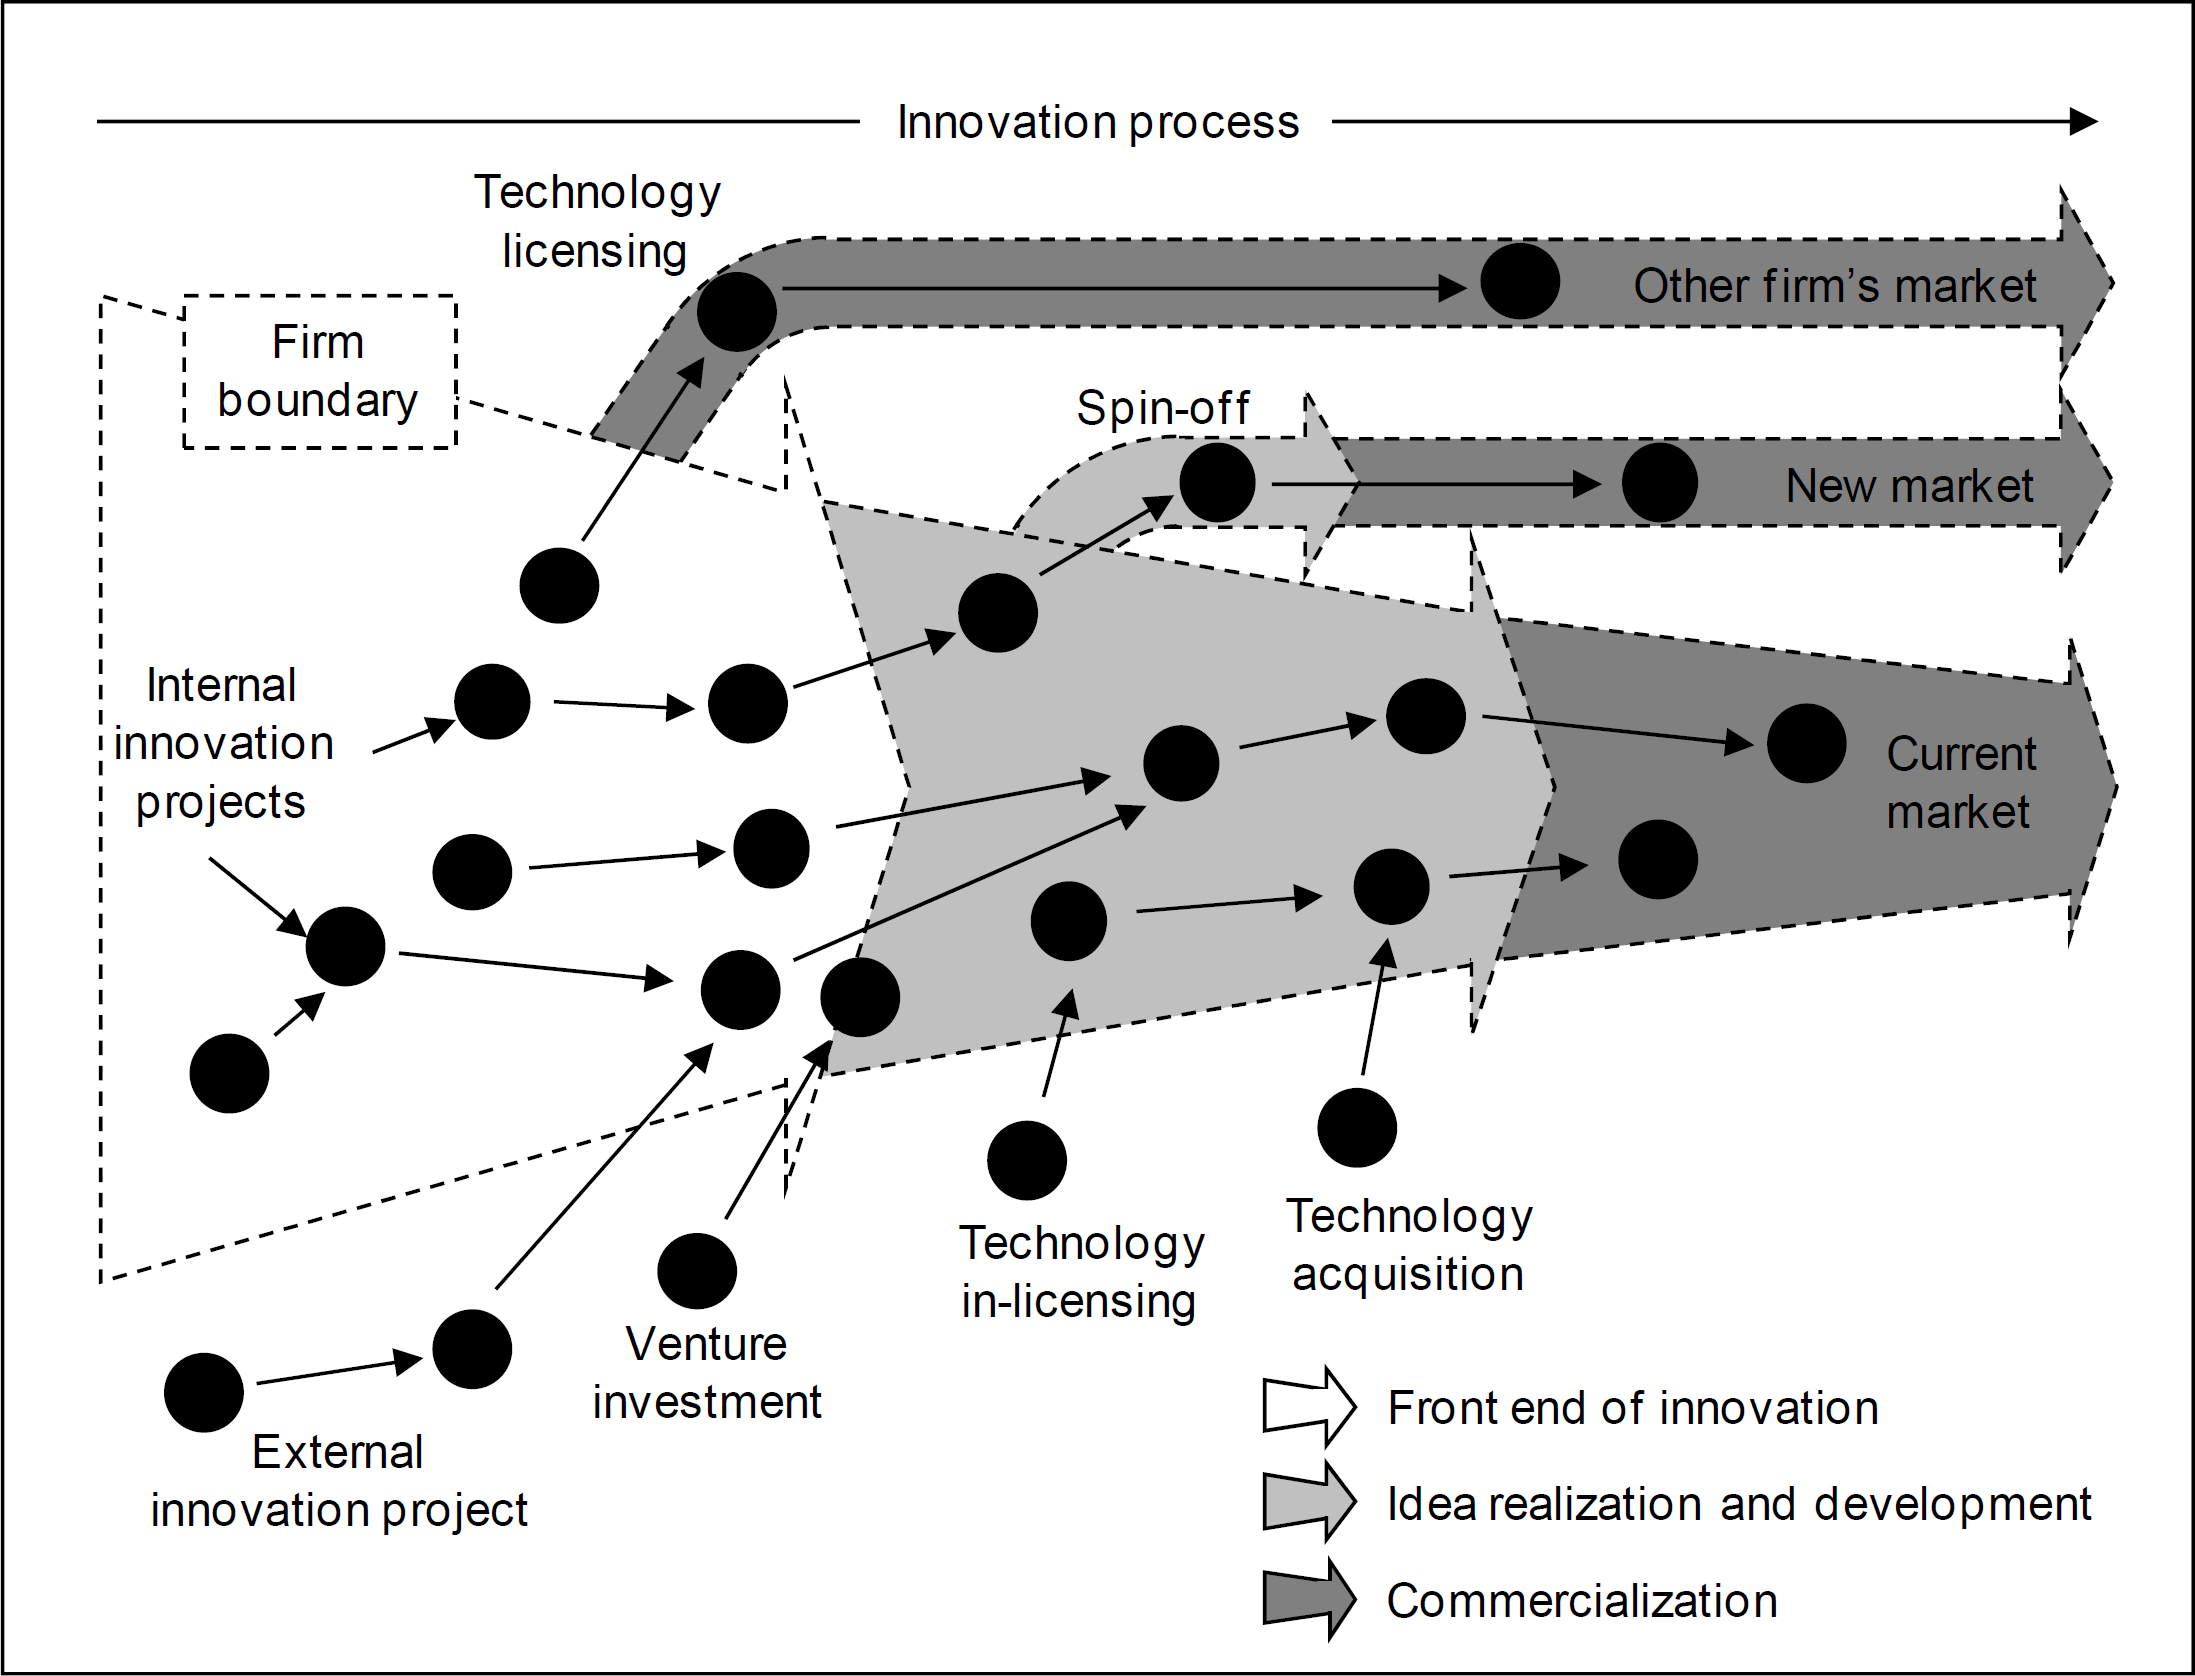
\includegraphics[width=1\textwidth]{OpenInnovation}
    \caption{Open Innovation Modell (aus \cite[23]{herzog2011})}
    \label{fig:openInnovation}
\end{figure}

Wie in \autoref{fig:openInnovation} zu sehen,
sind in der \textit{Open Innovation} die Grenzen eines Unternehmens \enquote{löchrig}.
Zusätzlich zu den intern entstandenen und entwickelten Innovationen
fließt jederzeit wissen von außen in den Innovationsprozess ein.
Außerdem werden Projekte, welche innerhalb des Unternehmens nicht weiterverfolgt werden,
veröffentlicht oder genutzt um neue Märkte zu erschließen.

Details zum \textit{Open Innovation}-Ansatz können in unter Anderem
in \cite[60\psqq]{chesbrough2003} und \cite[21\psqq]{herzog2011} nachgelesen werden.